\documentclass[tikz,border=6pt]{standalone}
\usepackage[T1]{fontenc}
\usepackage{lmodern}
\usepackage{amsmath,amssymb}
\usetikzlibrary{arrows.meta,angles,quotes,calc,positioning}
\definecolor{axis}{HTML}{40515F}
\definecolor{grid}{HTML}{DDE4E8}
\definecolor{blue}{HTML}{3568D4}
\definecolor{coral}{HTML}{EF626C}
\definecolor{teal}{HTML}{2A9D8F}
\definecolor{gold}{HTML}{D89432}
\definecolor{purple}{HTML}{7357C8}
\tikzset{
  axisline/.style={axis, line width=.85pt, -{Stealth[length=3mm]}},
  guide/.style={axis!45, line width=.75pt, dashed},
  vector/.style={line width=1.5pt, -{Stealth[length=3mm]}},
  dot/.style={circle, fill=white, draw, line width=1.15pt, inner sep=2.15pt},
  label/.style={font=\large},
  smalllabel/.style={font=\normalsize}
}
\begin{document}

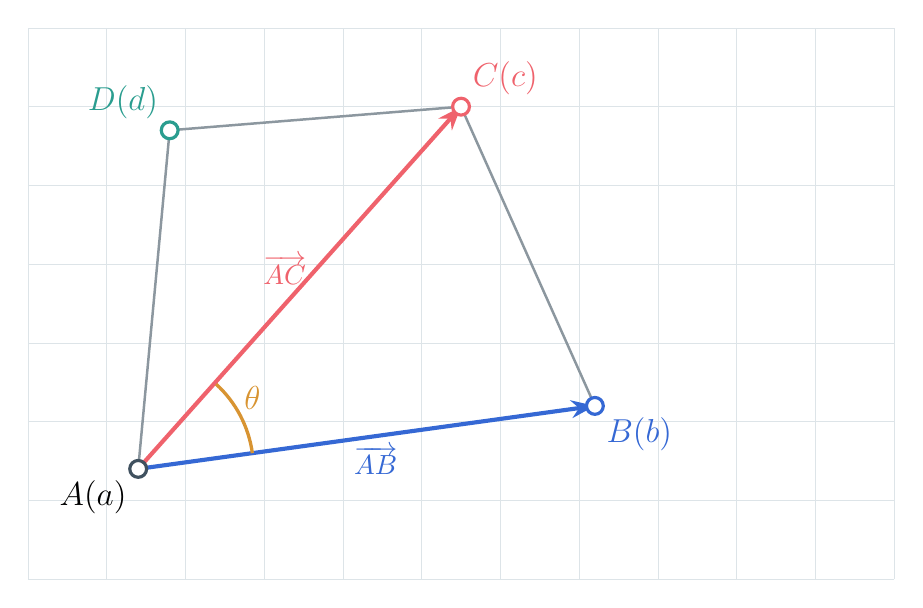
\begin{tikzpicture}[x=1cm,y=1cm]
  \draw[step=1cm,grid,very thin] (-1,-1) grid (10,6);
  \coordinate (A) at (0.4,.4);
  \coordinate (B) at (6.2,1.2);
  \coordinate (C) at (4.5,5);
  \coordinate (D) at (.8,4.7);
  \draw[vector,blue] (A)--(B);
  \draw[vector,coral] (A)--(C);
  \draw[axis!60,line width=.9pt] (B)--(C)--(D)--(A);
  \draw[gold,line width=1.2pt] ($(A)+(1.45,.2)$) arc[start angle=7.9,end angle=47.5,radius=1.46];
  \node[dot,draw=axis] at (A) {};
  \node[dot,draw=blue] at (B) {};
  \node[dot,draw=coral] at (C) {};
  \node[dot,draw=teal] at (D) {};
  \node[label,below left=1pt of A] {$A(a)$};
  \node[label,blue,below right=1pt of B] {$B(b)$};
  \node[label,coral,above right=1pt of C] {$C(c)$};
  \node[label,teal,above left=1pt of D] {$D(d)$};
  \node[label,gold] at (1.85,1.3) {$\theta$};
  \node[smalllabel,blue,below] at ($(A)!.52!(B)$) {$\overrightarrow{AB}$};
  \node[smalllabel,coral,left] at ($(A)!.55!(C)$) {$\overrightarrow{AC}$};
\end{tikzpicture}
\end{document}
